\def\code#1{\texttt{#1}}
\documentclass{SGGW-thesis}
\title{Projekt i~implementacja aplikacji mobilnej wyświetlającej aktualne lokalizacje autobusów oraz tramwajów w~Warszawie}
\Etitle{Project and implementation of mobile application displaying present locations of busses and trams in Warsaw}
\author{Bartosz Matyjasiak}
\date{2020}
\university{Szkoła Główna Gospodarstwa Wiejskiego\\w Warszawie}
\dep{Instytut Informatyki Technicznej}
\album{185117}
\thesis{Praca dyplomowa inżynierska}
\course{Informatyka}
\promotor{dr\ hab.\ inż.\ Leszek Chmielewski, prof.\ SGGW}
\pworkplace{Instytut Informatyki Technicznej\\Katedra Sztucznej Inteligencji}

\usepackage{hyperref}
\usepackage{graphicx}
\bibliographystyle{plain}

\begin{document}
\maketitle
\statementpage
\abstractpage
{Projekt i~implementacja aplikacji mobilnej wyświetlającej aktualne lokalizacje autobusów oraz tramwajów w~Warszawie}
{
Tematem niniejszej pracy było wykonanie aplikacji mobilnej pozwalającej w łatwy sposób odnalezienie autobusu lub tramwaju na mapie przy pomocy dostępnego publicznie API Warszawy.
Praca zawiera opis implementacji najważniejszych aspektów aplikacji.
}
{komunikacja miejska, mapa, implementacja, React-Native}
{Project and Implementation of Mobile Application Displaying Present Locations of Busses and Trams in Warsaw}
{
The subject of this study was to create mobile app that allows, in easy way, to find bus or tram on a map by using public API of Warsaw.
The thesis consists implementation descriptions of most important aspects of that mobile application.
}
{public transport, map, implementation, React-Native}


{
  % Spis treści może być złożony z~pojedynczą interlinią, np. jeśli jedna linia wychodzi na następną stronę.
  % W~przeciwnym razie spis treści wstawić bez powyższego rozkazu i~klamry.
  \doublespacing
  \tableofcontents
}

\startchapterfromoddpage % niezależnie od długości spisu treści pierwszy rozdział zacznie się na nieparzystej stronie


\chapter{Wstęp}
% po co taka aplikacja
W dużych miastach komunikacja miejska jest kluczowym aspektem dla mieszkańców.
Niestety duże miasta, w~tym Warszawa, boryka się z~korkami, wypadkami, robotami drogowymi i~innymi problemami, przez
co autobusy czy tramwaje często nie jeżdżą dokładnie według rozkładu jazdy.
Dlatego dobrą informacją dla podróżującego jest lokalizacja GPS autobusu lub tramwaju.
Warszawa udostępnia takie dane w~projekcie ,,Otwarte Dane''~\cite{APIWARSZAWA}, jednak są one w~postaci nieczytelnej dla przeciętnego człowieka.
Rozwiązaniem może być aplikacja mobilna, dzięki której użytkownik będzie widział na mapie, kiedy dokładnie przyjedzie autobus lub tramwaj.
% Dzięki temu też będzie wiedział, czy powinien się pospieszyć idąc na przystanek.
\section{Założenia}
% wymienić parę wymagań dla takiej aplikacji
% motywy
% aktualne pozycje 
% możliwość sprawdzenia rozkładu jazdy na danym przystanku
% dodawanie do ulubionych przystanków i~linii
Aplikacja powinna:
\label{ZALOZENIA}
\begin{itemize}
  \item{pokazywać aktualne pozycje autobusów i~tramwajów na mapie,}
  \item{pokazywać pozycje przystanków na mapie,}
  \item{udostępniać rozkłady jazdy na każdym z~przystanków,}
  \item{umożliwiać na dodanie linii autobusowej lub tramwajowej do ulubionych,}
  \item{umożliwiać na dodanie przystanku do ulubionych,}
  \item{wspierać dwa motywy:}
  \begin{itemize}
    \item{jasny,}
    \item{ciemny.}
  \end{itemize}
\end{itemize}
\vfill
\pagebreak
\section{Grafiki koncepcyjne}
By przybliżyć wizje projektu wykonałem grafiki koncepcyjne w~programie Figma.
Są to Rys.~\ref{koncept.ekran_glowny} i~Rys.~\ref{koncept.dolny_przybornik}.
\begin{figure}[!htb]
  \centering
  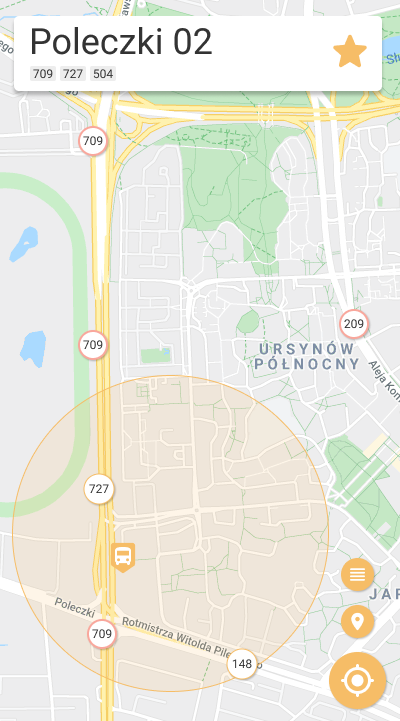
\includegraphics[width=75mm]{koncepty/screen_day_click_stop}
  \enspace
  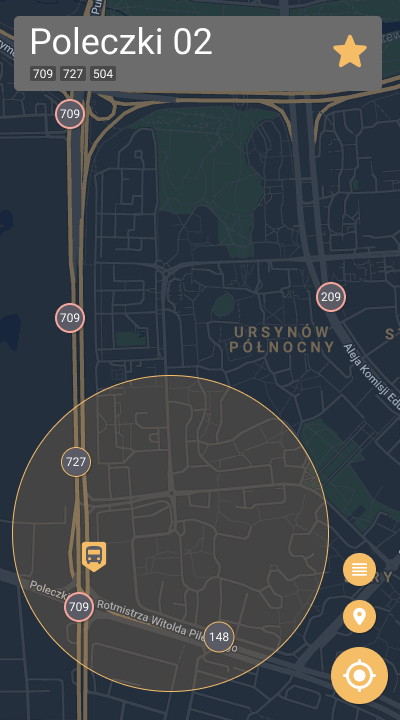
\includegraphics[width=75mm]{koncepty/screen_night_click_stop}
  \caption[Ekran główny - koncept]{
    \label{koncept.ekran_glowny}
    Grafiki koncepcyjne ekranu głównego z~wyświetlonym radarem, zaznaczonym przystankiem i~przykładowymi autobusami. Od lewej: motyw jasny, motyw ciemny. \vspace{2ex}
  }
\end{figure}
\begin{figure}
  \centering
  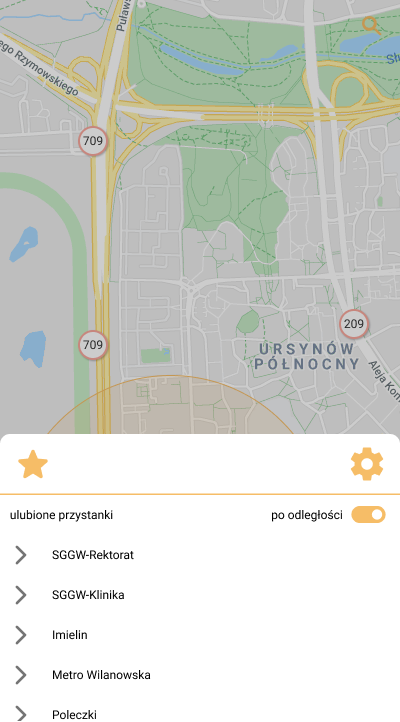
\includegraphics[width=75mm]{koncepty/screen_day_home_menu_click}
  \enspace
  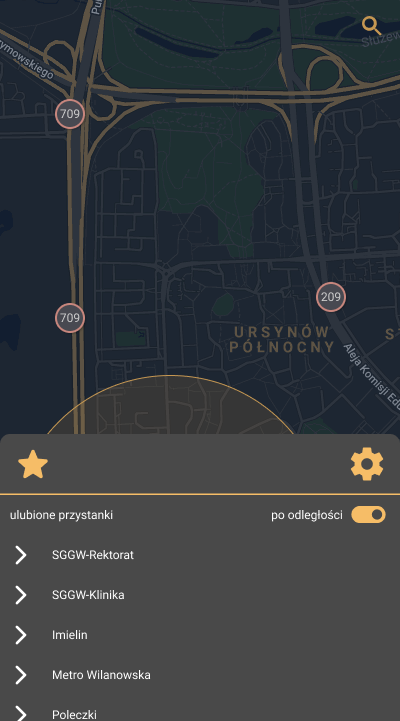
\includegraphics[width=75mm]{koncepty/screen_night_home_menu_click}
  \caption[Dolny przybornik]{
    \label{koncept.dolny_przybornik}
    Grafiki koncepcyjne dolnego przybornika z~ulubionymi przystankami. Od lewej: motyw jasny, motyw ciemny. \vspace{2ex}
  }
\end{figure}

\chapter{Implementacja}
% o~wybranym react nativie, o~paczce od map do reacta
Do implementacji wybrałem \textit{framework} React-Native stworzony przez firmę Facebook~\cite{REACT}.
Pozwala on na stworzenie aplikacji mobilnej z~systemem Android lub iOS przy pomocy jednego kodu źródłowego w~języku JavaScript XML (w skrócie JSX).
Skupię się jednak na wersji aplikacji na system Android.
Wybrałem także moduł \code{react-native-maps}~\cite{REACTMAPS}, który jest odpowiedzialny za wyświetlanie mapy Google oraz zarządzanie nią.

\section{Publiczne API Warszawy}
% TODO: odnośniki do plików dokumentacji tych endpointów
Miasto udostępnia dane w~postaci publicznego API.
Z~pośród wielu punktów końcowych interfejsu API Warszawy są dostępne:
\begin{itemize}
  \item{pozycje pojazdów danej linii;}
  \item{zbiór linii, które odjeżdżają z~danego przystanku;}
  \item{rozkład jazdy dla danej linii z~danego przystanku;}
  \item{zbiór wszystkich przystanków.}
\end{itemize}
Pozycje pojazdów są aktualizowane co 10 sekund i~też z~taką częstotliwością są aktualizowane w~aplikacji.
Wszystkie z~wymienionych punktów końcowych interfejsu API zaimplementowałem w~klasie \code{WarsawAPI}.


\section{Komponent GlobalContextProvider}
% TODO: odnośnik do Contextu w~React
W React-Native wszystkie elementy, które wyświetlają się na ekranie są komponentami.
Komponenty pomiędzy sobą są połączone relacją rodzic-dziecko.
Niesie za sobą to pewne problemy.
Jednym z~nich jest tzw.~\textit{prop-drilling}\footnote{Przekazywanie parametrów w dół poprzez wiele poiomów dziedziczenia. Dla wielu terminów trudno jest podać polski odpowiednik. W takich przypadkach, z braku lepszego rozwiązania, będziemy się posługiwać terminami angielskimi.}. % czy wyjaśniać czym jest?
By tego uniknąć użyłem kontekstu dostępnego w~React i~stworzyłem komponent \code{GlobalContextProvider} odpowiedzialny za całą logikę aplikacji.
Komponent ten przechowuje zmienne:
\begin{itemize}
  \item{zbiór wszystkich przystanków,}
  \item{zbiór ulubionych linii,}
  \item{zbiór ulubionych przystanków,}
  \item{aktualny wyświetlany region mapy,}
  \item{pozycje radaru oraz jego promień,}
  \item{zaznaczony przystanek lub pojazd.}
\end{itemize}
Oraz funkcje do modyfikacji tych zmiennych. %czy wymienić je? jest ich z~7
Komponent też przechowuje referencje do komponentu mapy oraz udostępnia funkcje od sterowania nią.
\begin{itemize}
  \item{Dopasowanie regionu mapy do grupy przystanków.}
  \item{Wycentrowanie mapy na lokalizacji GPS użytkownika.}
  \item{Zaznaczenie pojazdu lub przystanku i~wycentrowanie mapy na zaznaczoneniu.}
\end{itemize}

Jednak nie umieściłem w~nim logiki aktualizowania pozycji pojazdów, gdyż każda zmiana stanu
tego komponentu powoduje ponowne wyrenderowanie wszystkich komponentów \code{GlobalContext.Consumer}, a~wraz nim wszystkich jego dzieci.
Przez to, że ten komponent jest używany w~wielu miejscach to każda aktualizacja pozycji pojazdów, a~ta
jest co 10 sekund, powodowałaby ponowne wyrenderowanie całej aplikacji.
To wiązałoby się z~utratą na szybkości działania.

\section{Aktualizacja pozycji pojazdów}
% napisać o~funkcji API której użyłem do tego celu
% że co 10 sek
% odpytuje wszystkie linie z~ulubionych i~dodaje do wyniku wszystko
% odpytuje wszystkie linie z~radaru, które nie są w~ulubionych i~dodaje tylko
%   te, które są w~zasięgu radaru
By aktualizacja przebiegała sprawnie, wraz z~wyświetlaniem logikę aktualizacji umieściłem w~komponencie \code{GMap}.
Jest to komponent, który jako dziecko posiada tylko komponent mapy.
Jest to ważne bo gdy tylko zmieni się stan komponentu \code{GMap}, a~ten będzie się zmieniał co 10 sekund, to wywoła to ponowne wyrenderowanie tylko komponentu map.
W tym komponencie zaimplementowałem funkcje, która:
\begin{enumerate}
  \item{dla każdej ulubionej lub wykrytej przez radar (opisany w~\ref{RADAR}) linii są pobierane pozycje pojazdów tych linii;}
  \item{jako pojazdy do wyświetlenia są brane pod uwagę tylko te pojazdy, które są z~linii ulubionej lub w~promieniu radaru oraz czas wysłania sygnału GPS nie jest starszy niż 6 minut;}
  \item{aktualizuje stan komponentu \code{GMap} pobranymi pojazdami.}
\end{enumerate}
Funkcja ta jest uruchamiana co 10 sekund za pomocą funkcji \code{setTimeout} wbudowanej w~język JavaScript.

\section{Pinezki przystanków}
Wiedza o~tym, gdzie znajduje się przystanek jest bardzo ważna dla użytkownika.
Jednak nie można ich wszystkich wyrenderować na mapie gdyż jest ich 6449 w~sieci ZTM (stan na sierpień~2019~\cite{ZTMSTATS}).
Taka ilość praktycznie spowodowała by, że aplikacja nie nadawałaby się do użytku.
Dlatego zoptymalizowałem to w~następujący sposób.

\label{FIREBASE}
% pobieranie pliku z~firebasa, przygotowanego (tu o~grupach)
% tu napisać ze odrazu ten plik już ma pogrupowane przystanki po id
%   by zoptymalizować (i o~tym ze grupa ma tez wyliczoną średnią pozycje)
% tu opisac logike wyswietlania
Stworzyłem skrypt, który grupuje otrzymane przystanki z~API Warszawy po numerze zespołu przystanka oraz wylicza średnią pozycje przystanków grupy.
Wynik zapisuje do pliku \code{.json}.
Ze względów optymalizacyjnych i~możliwej przyszłej rozbudowy aplikacji plik ten hostuje w~serwisie Firebase.
Na tym serwisie też stworzyłem punkt końcowy interfejsu API, który zwraca ten plik.
Aplikacja przy uruchomieniu pobiera go.

%napisać mechanizm wyswietlania, te zoomy itd
Dzięki zmiennej \code{mapRegion} dostępnej w~komponencie \code{GMap} mogę ograniczyć pinezki do wyświetlenia.
Zmienna \code{mapRegion} przechowuje aktualnie wyświetlany region mapy i~posiada cztery następujące wartości:
\begin{itemize}
  \item{\code{latitude} -- szerokość geograficzna w~centrum wyświetlanego regionu mapy,}
  \item{\code{longitude} -- długość geograficzna w~centrum wyświetlanego regionu mapy,}
  \item{\code{latitudeDelta} -- różnica szerokości geograficznych od lewej krawędzi mapy do prawej,}
  \item{\code{longitudeDelta} -- różnica długości geograficznych od górnej krawędzi mapy do dolnej.}
\end{itemize}
Używając tych czterech wartości można przefiltrować pinezki i~wyświetlić tylko te, które są w~obrębie \code{mapRegion}.
Ponieważ, że zmienna \code{mapRegion} aktualizowana jest tylko kiedy manipulacja mapą (przesuwanie, obracanie itp.) zostanie zakończone to użytkownik nie zobaczy pinezek,
które w~trakcie ruchu weszły w~obręb wyświetlanego regionu mapy.
By polepszyć doświadczenie użytkownika (ang.~\textit{user experience}) do filtracji pinezek używam czterokrotnie większego pola niż pole wyznaczone przez \code{mapRegion}

By jeszcze bardziej ograniczyć ilość pinezek stworzyłem trzy progi wyświetlania zależne od wartości \code{latitudeDelta}:
\begin{enumerate}
  \item{$[0;0.02)$ -- wyświetla pinezki pojedynczych przystanków,}
  \item{$[0.02; 0.035)$ -- wyświetla pinezki grup przystanków,}
  \item{$[0.035;\infty)$ -- nie wyświetla żadnych pinezek przystanków.}
\end{enumerate}


Pinezki przystanków i~grup przystanków różnią się tylko wielkością oraz wyglądają jak na Rys.~\ref{screen.pin_przystanki}.
Kliknięcie w~pinezkę grupy przystanków dopasuje wyświetlany region mapy do wszystkich przystanków w~grupie,
a~w~pinezkę pojedynczego przystanku zaznaczy go.
\begin{figure}
  \centering
  
\includegraphics[width=15mm]{screeny/busstop_jasny}
  \enspace\enspace
  
\includegraphics[width=15mm]{screeny/busstop_ciemny}
  \caption[Pinezki przystanków]{
    \label{screen.pin_przystanki}
    Pinezki przystanków lub grup przystanków. Od lewej: motyw jasny, motyw ciemny. \vspace{2ex}
  }
\end{figure}


\label{RADAR}
\section{Radar}
% napisać, że zbiera linie z~przystanków które są w~granicach radaru 
Autobusów i~tramwajów w~Warszawie jest zbyt duża ilość by efektywnie pokazać je wszystkie na raz na mapie, więc dodałem do aplikacji funkcje radaru.
Głównym celem radaru jest pokazywanie pinezek pojazdów linii z~poza ulubionych.
Ogranicza on też ilość pinezek do narysowania.

Działanie radaru jest następujące:
\begin{enumerate}
  \item{użytkownik za pomocą przycisku w~prawym dolnym rogu ustawia pozycje radaru na środku regionu mapy, który jest aktualnie wyświetlany;}
  \item{dla każdego z~grup przystanków jest sprawdzane, czy średnia pozycja grupy jest w~promieniu radaru;}
  \item{jeśli tak to wszystkie linie z~każdego przystanka danej grupy są dodawane do zbioru unikalnych linii radaru.}
\end{enumerate}
% tu napisać o~tym hacku z~firebasem (tu napisać ze ze względu na 573925 zapytań o~linie jakie są
% na danym przystanku)
Podczas implementacji zauważyłem problem.
Jeśli w~granicach radaru jest $n$ przystanków to tyle samo będzie zapytań do API Warszawy o~linie jakie odjeżdżają z~danego przystanka.
Czas wysłania i~odbioru około średnio 40 zapytań był bardzo długi.
Dlatego do skryptu i~pliku opisanego w~\ref{FIREBASE} dodałem pobieranie dla każdego przystanka wszystkich linii oraz zapis ich do pliku wynikowego.



\section{Rozkłady jazdy}
By stworzyć możliwość sprawdzenia rozkładu jazdy dla danego przystanka postanowiłem dodać przycisk w~postaci ikony w~kontenerze u~góry ekranu po zaznaczeniu przystanka (patrz Rys.~\ref{screen.topbox}).
Po naciśnięciu aplikacja zmienia widok na liste odjazdów dla każdej z~linii (patrz Rys.~\ref{screen.rozklad_jazdy}).
Na rysunkach można zauważyć, że dodałem informacje na temat, ile czasu zostało do następnego odjazdu autobusu lub tramwaju.
Jest to czas z~zaokrągleniem do minut w~dół obliczony na podstawie rozkładu jazdy.
\begin{figure}[!htb]
  \centering
  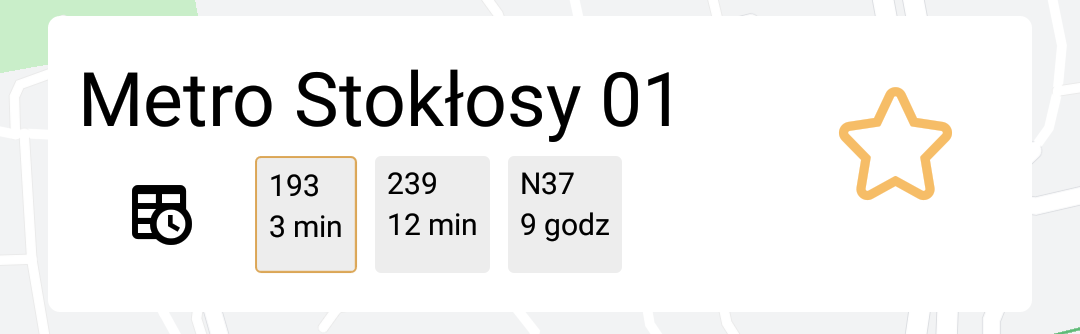
\includegraphics[width=75mm]{screeny/topbox_jasny}
  \enspace
  
\includegraphics[width=75mm]{screeny/topbox_ciemny}
  \caption[Górny kontener]{
    \label{screen.topbox}
    Górny kontener prezentujący informacje o~zaznaczonym przystanku. Od lewej: motyw jasny, motyw ciemny. \vspace{2ex}
  }
\end{figure}
\begin{figure}[!htb]
  \centering
  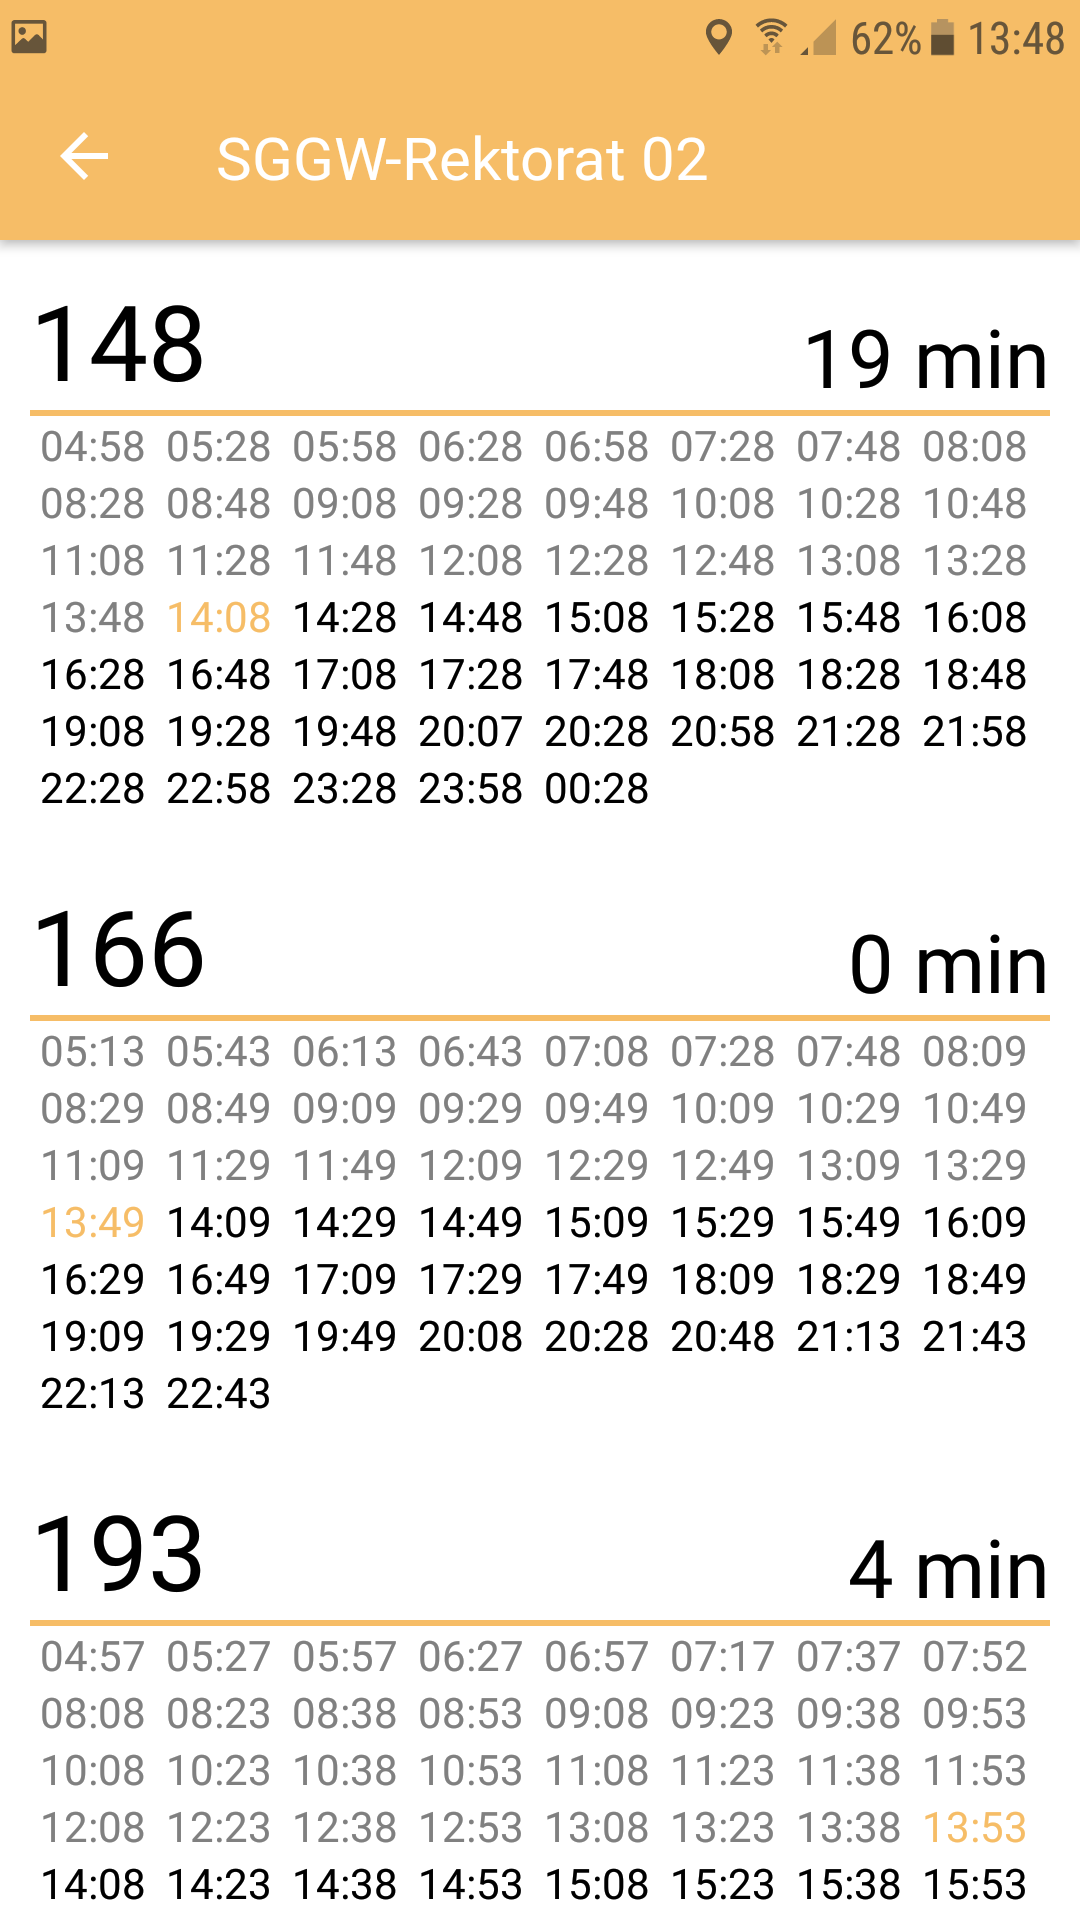
\includegraphics[width=75mm]{screeny/rozklad_jasny}
  \enspace
  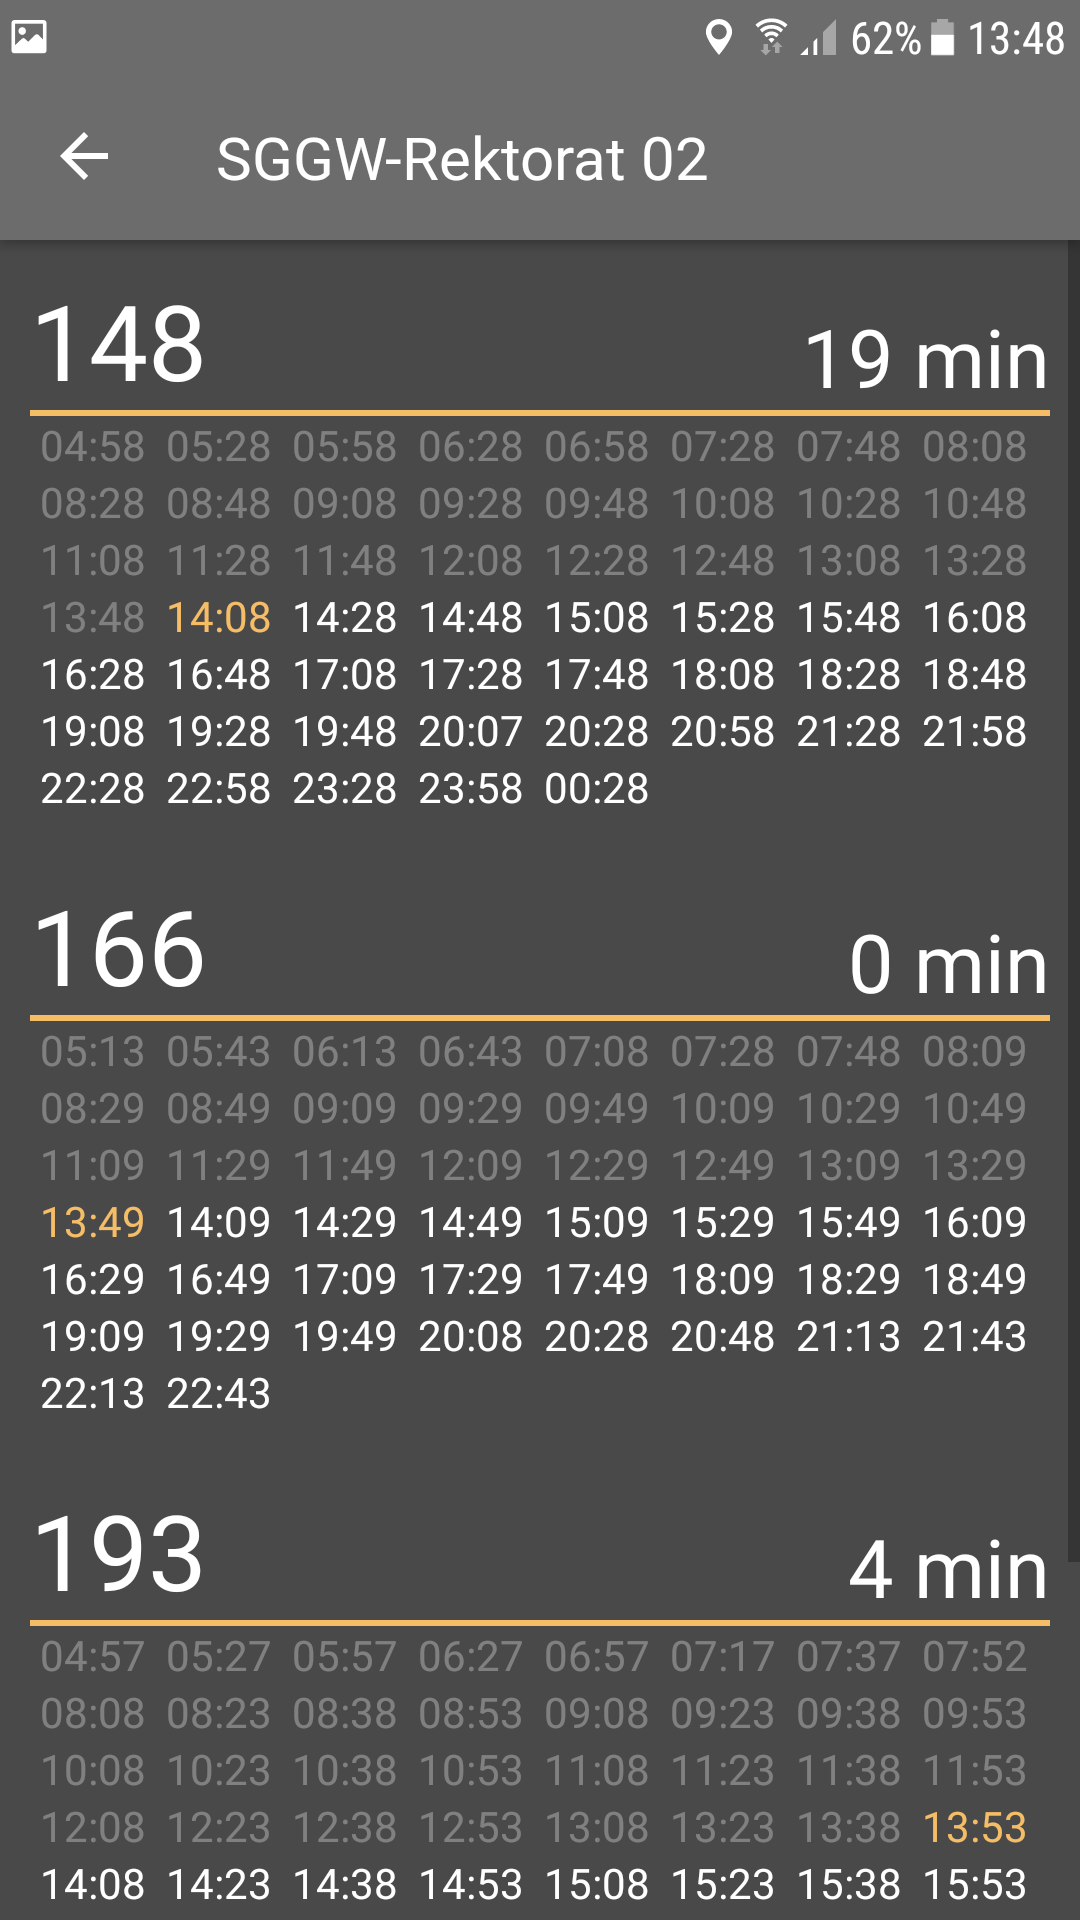
\includegraphics[width=75mm]{screeny/rozklad_ciemny}
  \caption[Rozkład jazdy]{
    \label{screen.rozklad_jazdy}
    Zrzut ekranu rozkładu jazdy. Od lewej: motyw jasny, motyw ciemny. \vspace{2ex}
  }
\end{figure}



\section{Ukrycie kluczy API}
% napisać że uzywam dwóch kluczy: do map i~do warszawskiego api
% że używam git'a do zarządzania zmianami w~kodzie
% i~że klucze nalezy ukrywać w~plikach np. .env
% a~ze do warsaw api poprzez BuildConfig z~paczki react-native-config
W aplikacji używam dwóch API: Warszawy oraz map Google.
Każde z~nich wymaga klucza API.
Te klucze powinny pozostać prywatne i~niewidoczne w~kodzie aplikacji.
Dlatego by ukryć klucze stworzyłem plik \code{.env} w~lokalizacji domowej projektu, w~którym zdefiniowałem dwie zmienne środowiskowe:
\code{WARSAW\_API\_KEY} oraz \code{GOOGLE\_MAPS\_API\_KEY} o~odpowiednich wartościach.

Następnie w~kodzie posługiwałem się zmienną \code{BuildConfig} z~modułu \code{react-native-config}~\cite{REACTCONFIG} by otrzymać klucz API Warszawy,
a klucz map Google, należało umieścić w~pliku \code{AndroidManifest.xml} przy pomocy odwołania do zmiennych środowiskowych (ang.~\textit{build variables}) po uprzedniej konfiguracji modułu \code{react-native-config} i zmiennych w pliku \code{build.gradle}.

Po wykonaniu tych operacji można bezpiecznie użyć systemu kontroli (np.~"git") i~serwisów jak GitHub do udostępniania kodu.
Należy też dodać lokalizacje pliku \code{.env} do pliku \code{.gitignore}.
Teraz by było możliwe zbudowanie aplikacji w~trybie debug należy wypełnić plik \code{.env.example} własnymi kluczami i~zmienić jego nazwę na \code{.env}.


\chapter{Podsumowanie i~wnioski}
Stworzono aplikacje mobilną spełniającą założenia przedstawione w~sekcji~\ref{ZALOZENIA}.
Końcowo ekran główny aplikacji wygląda jak na Rys.~\ref{screen.glowny}.
Funkcje aplikacji pozwalają na szybkie korzystanie z~niej przez użytkownika po dodaniu linii i~przystanków do ulubionych.
Aplikacja posiada też spore możliwości rozwoju, takie jak przewidywanie czasów przyjazdu, kupowanie biletów lub wyświetlanie tras przejazdu danych linii autobusowych lub tramwajowych.
Dzięki zastosowanej technologii React-Native, isnieje możliwość dość łatwej rozbudowy aplikacji na systemy iOS.
\begin{figure}
  \centering
  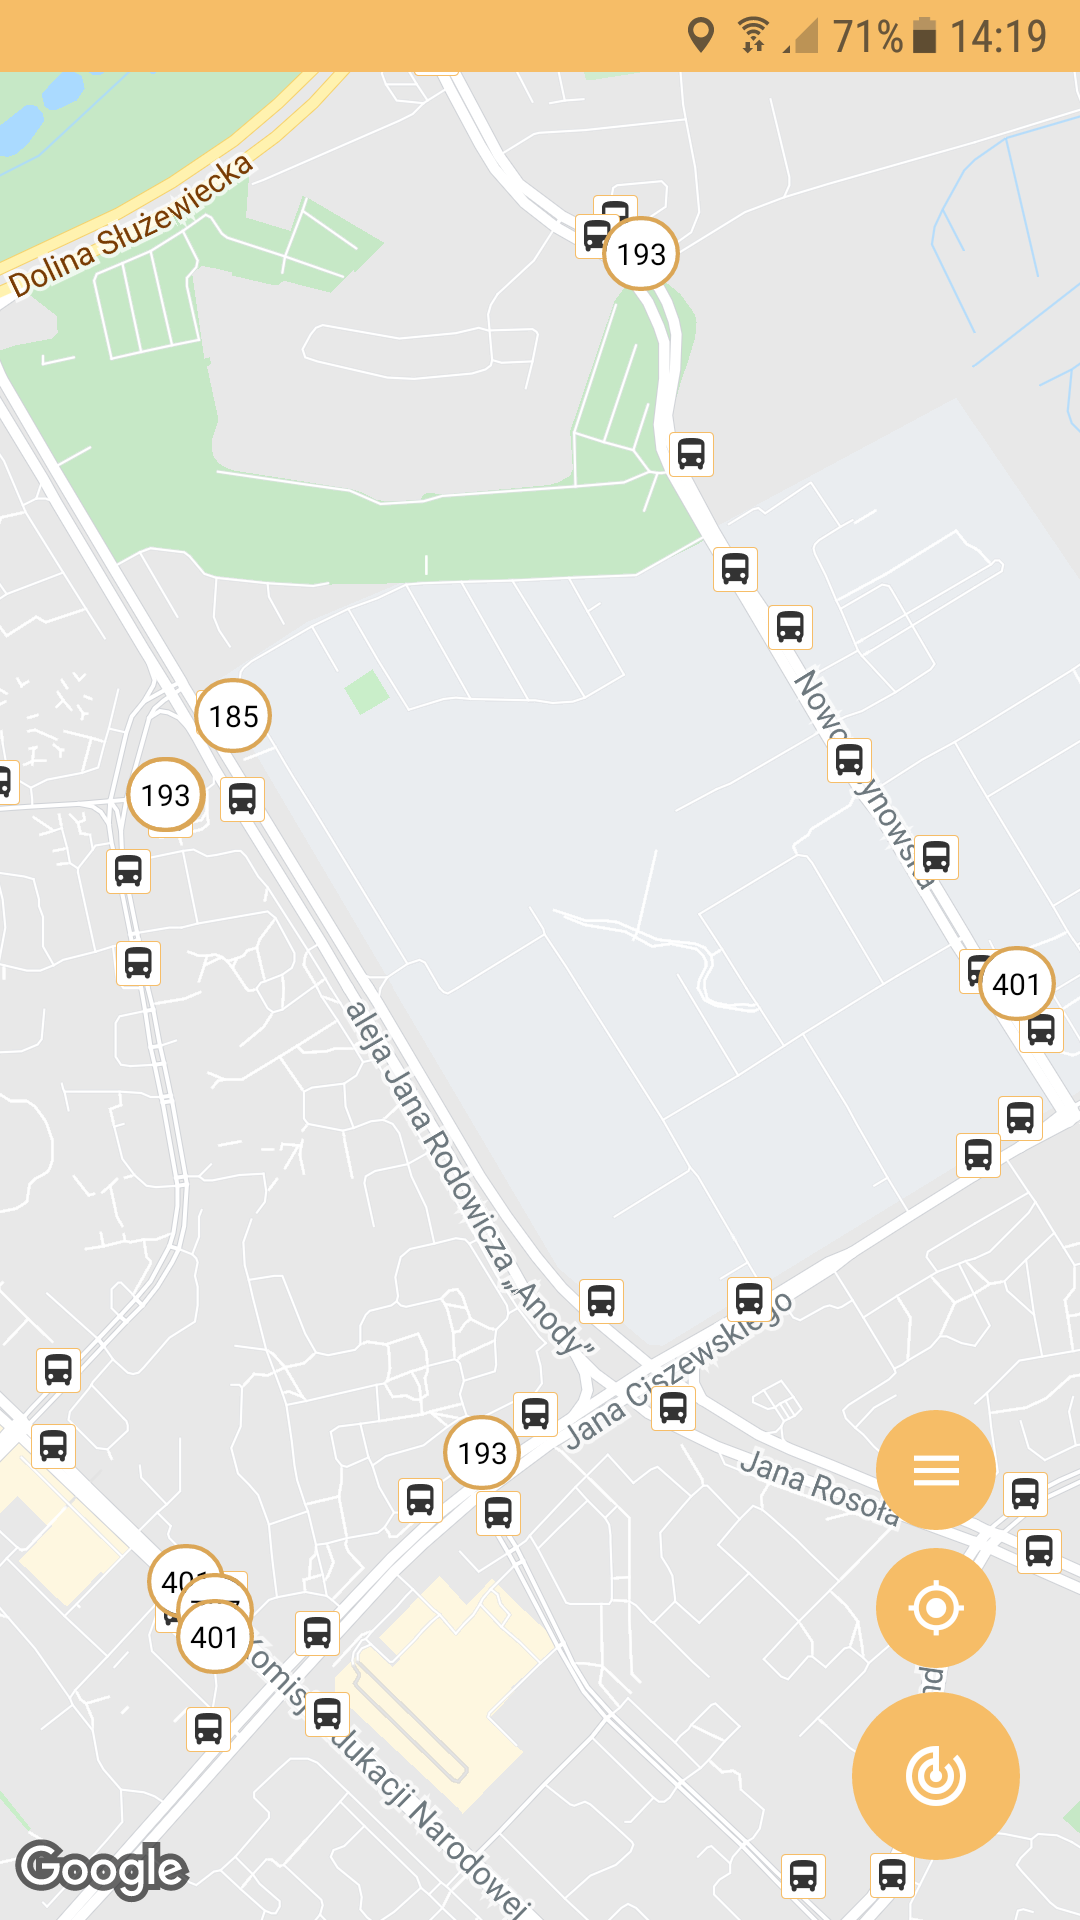
\includegraphics[width=75mm]{screeny/glowny_jasny}
  \enspace
  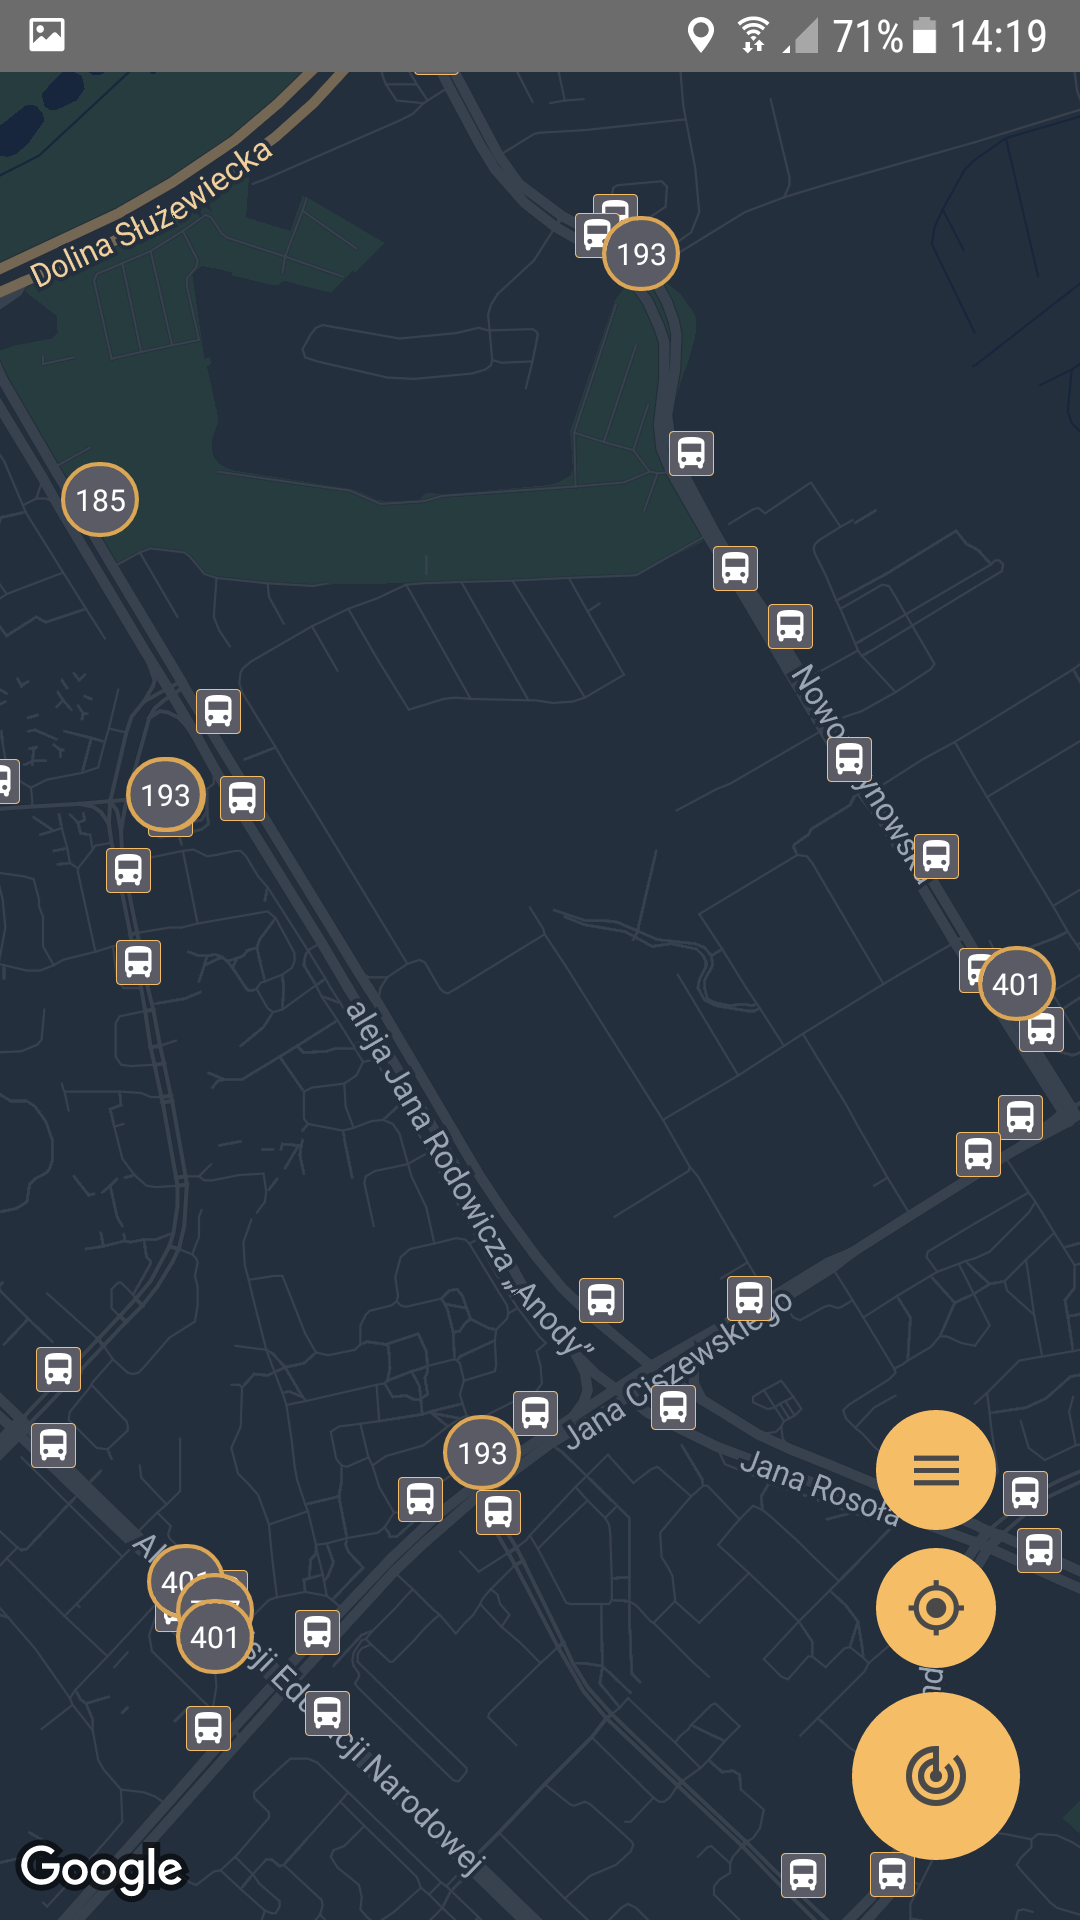
\includegraphics[width=75mm]{screeny/glowny_ciemny}
  \caption[Ekran główny]{
    \label{screen.glowny}
    Zrzut ekranu głównego aplikacji. Od lewej: motyw jasny, motyw ciemny. \vspace{2ex}
  }
\end{figure}

\bibliography{bib0}

\beforelastpage

\end{document} 